%% This is the chapter 1. This chapter will need to be translated from a word document to the Latex.
%% It will give a little more of work. Not that much, I think.

\chapter{HAVE CORAL SNAKE MIMICS DIVERSIFIED MORE THAN NON-MIMICS?}

\section{Abstract}

Dipsadidae is one of the most diversified family of snakes, composed of species showing an impressive variety of color patterns. Some species are cryptic whereas others have contrasting patterns comprised by bright colors alternated with darker shades, including particular combinations of vivid colors characteristic of coral snakes (Elapidae). Species with such patterns are thought to be mimics of coral snakes based on their color pattern similarity, predator avoidance of such patterns in field experiments, and the geographical concordance between models and mimics. Here we test whether color patterns associated with coral snake mimicry and contrasting color patterns in general influenced the diversification dynamics of the group. We compile a large database of color patterns with color descriptions for about 80\% of the known diversity of the group (594 species). We used trait-dependent diversification models along with extensive simulations to deal with the recently described statistical bias associated with such methods. We also tested whether color patterns are associated with trait-independent estimates of diversification. Despite the apparent survival advantage associated with coral snake mimicry, we show that there is no detectable influence of color types in the dynamics of diversification in Dipsadidae and discuss insights into the potential functions of color patterns.

\section{Introduction}

Colors play an important role in avoiding predation. Patterns similar to the background environment make prey difficult for the predators to detect and recognize \citep{merilaita_2005, stevens_2009}. On the other hand, bright and contrasting colors displayed by unpalatable, toxic or venomous animals (i.e., aposematic patterns) serve as warning signals that are often avoided by visually oriented predators \citep{wallace_1867, mappes_2005, speed_2005}. However, such conspicuous colors can also be displayed by mimics, which gain protection by deceiving predators that avoid their false warning signals. Strong evidence from field experiments shows that mimicry of warning signals decreases predation pressure when compared to cryptic color patterns \citep{jeffords_batesian_1979, brodie_differential_1993, brodie_experimental_1995, pfennig_2001, pinheiro_2011, pfennig_2015}. Such reduction in predation pressure may also have positive impacts on habitat use by aposematic lineages and their mimics. Cryptic animals are to some degree restricted to backgrounds which their color patterns match and may only be active at certain times because movement is often antithetic to good crypsis \citep{speed_2010, stevens_2012}. In contrast, such restrictions may be weaker in aposematic or mimic lineages, which could promote more opportunities to exploit habitat resources \citep{speed_2010}.

In contrast with aposematism, the survival advantage of Batesian mimicry is dependent on the relationship between the model and the mimetic organism because predators need to associate the unpalatability or hazard of the model with the warning signals of the deceiver. Once this association is broken, a mimicry breakdown occurs and the mimic phenotype might become maladaptive since warning signals can make individuals more conspicuous to predators \citep{mallet_evolution_1999, pfennig_2001, pfennig_2015}. Mimicry breakdown can be caused by allopatry between mimic and model populations as a result of population expansion of the mimic or local extinction of the model \citep{pfennig_2010}. Allopatric mimics are conspicuous to naïve predators that might not avoid their deceptive warning signals and this may result in higher predation rates and eventual extinction of the mimic population \citep{pfennig_2015}. On the other hand, population expansion or migration of mimics can create opportunities for local adaptation to novel aposematic models. This process could result in selection against intermediate hybrids followed by decreased gene flow among populations and eventually promote reproductive isolation \citep{mallet_evolution_1999, pfennig_2015}. Over longer time scales such processes might have a positive effect on rates of diversification of mimetic lineages. Previous studies show that aposematic lineages are more species-rich than cryptic ones \citep{santos_2003, przeczek_2008}, suggesting that the evolution of the aposematic condition may even represent a key innovation \citep{speed_2010}. This key innovation hypothesis could be extended to mimicry; however, the potential effects of mimicry evolution on lineage diversification have yet to be investigated.

Among snakes, groups of relatively harmless or mildly venomous species showing color patterns similar to those of venomous coral snakes (Elapidae) have instigated a long debate on whether such patterns are mimetic \citep[see a comprehensive review in][]{pough_1988}. Reports often rely on the similarity of color patterns between mimics and models to argue in favor of mimicry relationships \citep{dunn_coral_1954, hecht_coral_1956, greene_coral_1981, savage_1992}. Additional evidence come from parallel geographic variation of coral snakes and their putative mimics \citep[e. g.,][]{hecht_coral_1956, zweifel_1960, greene_coral_1981, marques_1991, rabosky_coral_2016} and from field studies using replicas of coral snakes and other similar color patterns \citep{smith_1975, brodie_differential_1993, brodie_experimental_1995, hinman_predation_1997, pfennig_2001, buasso_predation_2006}.

Some authors pointed to the possibility that contrasting colors, including the stereotypical banded pattern observed in almost all coral snakes, could serve a disruptive function \citep{gadow_1908, thayer_1909, dunn_coral_1954, brattstrom_coral_1955}. Those reports suggested that the alternate pattern of bands could blend to the background environment and break the outline of the snake body, making recognition by visually oriented predators difficult. Recently, Titcomb and colleagues \citeyear{titcomb_2014} showed that the contrasting ringed pattern of coral snake mimics can create an illusory effect when the individuals are moving fast. The effect, called flicker-fusion, can give advantage to snakes against avian predators independent of mimicry. Despite its protective effect, the plausible disruptive function of the contrasting bands do not invalidate the existence of a mimicry complex between elapids and snakes from other families, since the same color pattern can perform both functions \citep{titcomb_2014}.

The family Dipsadidae (\citealp{zaher_2009}, \textit{sensu} \citealp{grazziotin_molecular_2012}) is a diverse group of snakes, with ca. 700 species occurring from Central to South America \citep{grazziotin_molecular_2012, uetz_2014}, and is characterized by an impressive variety of color patterns \citep[see][for some examples]{martins_1998}. Some dipsadids have color patterns similar to those of coral snakes, and have long been suggested as cases of mimicry of New World coral snakes \citep[family Elapidae;][]{wallace_1867, greene_coral_1981, sazima_1991, savage_1992, martins_1993, pough_1988, almeida_morphological_2014}. The contrasting coloration found in dipsadid snakes always includes bright colors but is not restricted to ringed patterns. In general, species can vary from the coral snake pattern of black, red and yellow rings or bands to a less colorful homogeneous red body with a single black or cream band on the neck (nuchal collar). Besides contrasting color patterns, the family also shows a diverse array of cryptic color patterns, characterized by blotches and shades of brown, gray, or green. Included in the latter are species whose dorsum is cryptic and whose venter has a plain bright color and even a coral snake pattern. Mimetic and cryptic patterns can be found both within and among genera and make dipsadid snakes an ideal study system to investigate the possible effects of such distinct color types on macroevolutionary patterns.

Herein we test whether distinct color patterns have an influence on the diversification of the family Dipsadidae. We investigate whether color patterns similar to coral snakes (and contrasting color patterns in general) show diverging macroevolutionary patterns when compared to non-mimic and cryptic lineages, respectively. We show that there is no detectable influence of supposedly mimic or contrasting color patterns in the dynamics of diversification.

\section{Materials and Methods}

\subsection{Phylogenetic reconstruction}

We used sequence data for Dipsadidae and outgroup species previously analyzed by Grazziotin and colleagues (2012, see GenBank accession numbers in their Appendix S1). We aligned sequences using MAFFT \citep{katoh_mafft_2005} under the G-INS-i strategy and selected models of molecular evolution for each of the eight gene sequences using a decision theory framework in DT-ModSel \citep{minin_2003}. We concatenated the alignments and set four partitions; one partition for each nuclear gene (bdnf, c-mos, and rag2) and a single partition with the mitochondrial genes (12S, 16S, cytb, nd2, and nd4). We used phyutility \citep{smith_2008} to trim down all sites with 75\% or more missing data and inferred a Maximum Likelihood (ML) tree using GARLI 2.0 \citep{zwickl_2011}. We used the resulting ML phylogeny as the starting tree for three independent searches in BEAST 1.8 \citep{drummond_bayesian_2012} for 270 million generations with a thinning interval of 1500 generations each. Since there are sequences available for only few species of each genera we set an incomplete sampling birth-death tree prior \citep{stadler_2009} and an uncorrelated relaxed clock model to estimate relative branching times. We checked each run for convergence using Tracer 1.6 \citep{drummond_bayesian_2012} and excluded 50\% of the posterior chain as burnin. We then combined the posterior from the three BEAST searches and randomly sampled 100 trees, rescaled all trees to a total depth of 1, and retained only one randomly selected species of each genera while pruning the rest. When the original tree had paraphyletic genera we selected the most inclusive monophyletic clade representing each group and kept a single species to represent each of those genera. Then, we used the resulting pool of genus-level phylogenetic trees to perform all subsequent comparative analyses. The 100 sampled trees and the BEAST xml file comprising the data matrix, selected models of molecular evolution, starting tree and prior parameters is available in FigShare (http://dx.doi.org/10.6084/m9.figshare.831493). We also deposited the configuration and log files for GARLI 2.0. Figures \ref{fig:full_MCC1} and \ref{fig:full_MCC2} show the resulting maximum clade credibility (MCC) tree and respective posterior probability support values.

\subsection{Color patterns}

To understand the evolution of colors and its effect on diversification we compiled a large database of coloration patterns for dipsadid snakes. We searched several information sources such as comprehensive taxonomic reviews \citep[e.g.,][]{downs_1967}, published articles and books containing photographs of identified individuals \citep[e.g.,][]{savage_2002, campbell_lamar_2004}, trusted on-line photo repositories (e.g., CalPhotos - http://calphotos.berkeley.edu/ and Reptile Database – \citealp{uetz_2014}), photographs of live individuals, and museum specimens. We excluded invalid taxa or names presenting nomenclatural problems that are still appearing in the literature or online databases. We avoided subspecific ranks for coding the currently recognized taxa (with the exception of four subspecies of \textit{Alsophis antillensis}) because terminals in available phylogenies correspond to species only and less than 10\% of the members of the family Dipsadidae present valid subspecies to date.

While color diversity makes the family Dipsadidae interesting for studies focusing on the evolution of color patterns such as ours, this is also the most challenging characteristic of the system. Since it is not possible to consider all diversity of color patterns for comparative analyses, we used categories that are directly related to the hypotheses tested. For that, we describe below two distinct classifications of the color patterns, each one including a different important aspect of the biology of the group. We repeated all comparative analyses with each of these color pattern classifications in order to access how distinct interpretations of color diversity in the group affect our macroevolutinary conclusions.

First, we compared coral-mimics with non-mimics. We call coral-mimics species that resemble the color pattern of any New World coral snake species \citep[see][]{roze_1996, campbell_lamar_2004}. Species included in this category can show the coral-mimic pattern throughout the dorsum (e.g., \textit{Simophis rhinostoma}) or restricted to the anterior portion of the body (e.g., \textit{Pseudoboa coronata}). On the other hand, all species not defined as potential mimics of coral snakes, independent of whether their color pattern was better described as contrasting or cryptic, were included in the category of non-mimics. As a result, the non-mimic category comprise species with cryptic color patterns and others with bright coloration but not resembling any known lineage of New World coral snake. Second, we compared contrasting with cryptic species. We defined as contrasting species that show brightly colored patterns in general, independent of whether the color pattern was similar to those of coral snakes. The category coral-mimic is a subset of the contrasting category; every coral-mimic lineage is among the species defined as contrasting, but the reverse is not true. On the other hand, we defined as cryptic all color patterns lacking contrasting colors. Examples of such patterns are blotches with hues of brown, reddish brown, gray, and other combinations of dark colors. We also considered as cryptic species whose dorsum is homogeneously green, since individuals of those species are usually found among leaves of trees and bushes (e.g., \textit{Uromacer}).

There are three other important aspects of the color patterns in the group that could potentially affect our study; the presence of color polymorphism, ontogenetic changes in coloration and contrasting coloration restricted to the venter of the body. In the case of species with color polymorphism, some populations may show cryptic patterns occasionally associated to thermoregulation (\citealp{tanaka_2005}, but see \citealp{lorioux_2008}). Alternatively, contrasting colors in polymorphic populations can be due to increasing sexual dichromatism in the course of the reproductive season \citep{forsman_opposing_1995, lindell_1996}, related to non-selective processes, such as migration and dispersal \citep{king_color_1995} or genetic drift in local \citep{brakefield_genetic_1990} or island populations \citep{bittner_gene_2003}. Independent of the potential sources of the polymorphic color patterns we assigned species to the non-mimic and cryptic categories every time a cryptic morph was described among color types. Some Pseudoboini snakes \citep[\textit{sensu}][]{zaher_2009} show ontogenetic changes in color pattern in which juveniles are brightly colored but become cryptic when adults \citep{martins_1998}. We included those species into the contrasting category since juveniles correspond to the life stage most threatened by predation \citep{bonnet_dangers_1999} and thus their defensive tactics are fundamental for individuals to reach sexual maturity. Finally, some species show cryptic color patterns in the dorsum but have contrasting patterns restricted to the venter. The distinct patterns in the dorsum and venter are usually associated with a threatening display in which individuals twist the body and expose the bright colors when disturbed \citep{martins_1993, sawaya_2008, tozetti_2009}. Hence, we classified those cases into the contrasting category instead of following their dorsal coloration. We provide additional data with the list of species included in each of these cases. We also repeated comparative analyses with alternative color categories defined to accommodate such cases, but results showed no appreciable difference when compared to the coral-mimic vs. non-mimic or contrasting vs. cryptic categories.

\subsection{Comparative analyses}

In order to test whether color patterns influence the dynamics of diversification of Dipsadidae snakes we performed a series of complimentary phylogenetic comparative analyses using the pool of 100 trees sampled from the posterior distribution and the three distinct color pattern classifications defined above. We used the Binary State Speciation and Extinction model \citep[BiSSE –][]{maddison_2007, fitzjohn_estimating_2009, fitzjohn_2012} and the Hidden State Speciation and Extinction model \citep[HiSSE –][]{beaulieu_detecting_2016} followed by model adequacy simulations. Both BiSSE and HiSSE are joint models of trait and trees \citep{beaulieu_detecting_2016} because model parameters reflect diversification rates conditioned on the state of the traits and trait transitions throughout the tree. In addition, we estimated trait-independent diversification rates using BAMM \citep{rabosky_2014} and tested whether the distribution of color patterns across dipsadid genera is associated with the diversification dynamics of the group. We describe details for each analyses below.

Since a species-level tree is not available for the Dipsadidae family, we used the pool of genus-level trees as terminally unresolved trees \citep[\textit{sensu}][]{fitzjohn_estimating_2009} to estimate trait-dependent diversification using BiSSE. We used Markov chain Monte Carlo (MCMC) to estimate the posterior distribution of the parameters for the unconstrained BiSSE model (six free parameters) and the constrained model, in which $\lambda$ and $\mu$ are not related to color types (four free parameters). We used an exponential prior distribution with rate parameter equal to 0.3 for all BiSSE parameters and a starting point equal to the maximum likelihood estimate (MLE) for the model. We ran 10,000 generations of MCMC (chain length was based on preliminary analyses), discarded 50\% of generations as burnin and checked convergence using the `coda' package \citep{plummer_2006}. To test whether the full model explained the data better than the trait-independent model we performed model selection using the Bayesian Deviance Information Criteria \citep[DIC –][]{gelman_understanding_2013}. In order to account for the behavior of the BiSSE model when its assumptions are violated \citep{rabosky_2015, beaulieu_detecting_2016}, we did posterior predictive checks for model adequacy to test whether data simulated under the trait-dependent and trait-independent BiSSE models are similar to the observed data. For each model, we simulated traits using the `tree.bisse' function in the package `diversitree' \citep{fitzjohn_2012} with parameters drawn from the joint posterior distribution resulting from the BiSSE analysis and constraining simulations to have a tree depth equal to 1 (identical to the empirical trees). Then, we compared the number of species and the relative frequencies of each trait generated by the simulations with the empirical dataset. If models are adequate, simulated phylogenies should produce both diversity and frequency of states similar to the observed data.

Recently, \citet{beaulieu_detecting_2016} described the HiSSE model that introduces hidden states associated with each of the traits and helps to accommodate the rate heterogeneity observed on empirical phylogenetic trees \citep{rabosky_2015, beaulieu_detecting_2016}. The implementation of HiSSE integrates incomplete sampling using the proportion of known species associated with each trait across the whole tree, but does not include the option of terminally unresolved phylogenetic trees such as `diversitree' \citep{fitzjohn_2012}. We fitted the 20 trait-dependent (including BiSSE and HiSSE models) and 4 trait-independent models to each of the 100 genus-level phylogenetic trees and performed model choice among models fitted for each tree using the Akaike Information Criteria (AIC).

Finally, we used BAMM \citep{rabosky_2014} to estimate rates of diversification and shift locations in the tree independent of the trait data. Different from the BiSSE and HiSSE analyses, we used species-level phylogenies by randomly resolving the relationships within each genera using a constant rate Birth-Death model \citep{kuhn_simple_2011}. This approach assumes that diversification rates are homogeneous within each genera but should not bias the estimation of diversification rates for the backbone tree, since BAMM fits distinct rate regimes to different parts of the tree. Additionally, we set the BAMM model with constant rates through time within each regime \citep[similar to MEDUSA –][]{Alfaro_2009}, since this is a more adequate model given that diversification rates within genera were constrained to a homogeneous clock model. We set two independent MCMC chains for each of the 10 phylogenetic trees randomly sampled from the BEAST analysis. We ran each chain for 5 million generations, discarded 20\% of generations as burnin and checked convergence using the `coda' package \citep{plummer_2006}. Finally, we tested for a linear relationship between diversification rates and the proportion of each color pattern among species of each genera. Since there is large variation in species richness across the genera, we performed two analyses; the first including all genera with at least two species and the second excluding all genera with less than 10 species (total of 54 and 14 genera, respectively).

Recently, Moore and colleagues \citeyear{moore_2016} pointed out some important issues with BAMM's implementation; that the likelihood function does not incorporate diversification shifts on unobserved branches of the tree, that posterior estimates of the number of shifts is sensitive to the prior specification and that use of the compound Poisson process (CPP) prior make it difficult to differentiate many rate shifts of small effect from fewer rate shifts of large effect. Shortly after, Rabosky and colleagues \citeyear{rabosky_2017} responded to the critiques by showing that not incorporating shifts on unobserved branches has only minor impacts on inferences and argued that \citet{moore_2016} assessment of prior sensitivity on posterior estimates of the number of shifts was problematic. In this study, we use only relative diversification rates compared across genera (i.e., the slope of the regression) and our analyzes do not focus on the posterior distribution of the number of rate shifts across the tree. Thus, we believe that most concerns associated with BAMM should not have major impacts on our biological conclusions. Nevertheless, we repeated BAMM analyses with different prior distributions for the expected number of shifts ($\gamma$ = 0.1, 1, or 10) to test whether our results could be affected by the prior sensitivity.

We repeated all trait-dependent analyses with each of the three distinct color pattern categories. R scripts, BAMM files, phylogenetic trees and coloration data to reproduce all analyses are available in the github repository \url{https://github.com/Caetanods/Dipsadidae_color_evolution} .

\section{Results}

We compiled a large report of coloration descriptions for 594 species of dipsadid snakes covering over 80\% of the known diversity of the group. We were able to get detailed color descriptions for most species, but for some the information available was incomplete or limited (i.e., taxa known from a single specimen). Although those cases were not suitable for definition as coral-mimic or non-mimic lineages (i.e., state unknown or `NA'), we managed to classify those as either contrasting or cryptic for all but a few exceptions. Among all data sources, museum specimens are the most difficult to categorize since colors fade after preservation and only light and dark hues remain. Bright colors such as yellow, orange, pink, and red (derived from carotenoid pigments) fade completely over time turning into cream on preservative fluid. In contrast, dark pigmentation is preserved and sometimes turns into shades of black or dark brown. As a result, we assigned museum specimens with alternate bright and dark bands (or with a distinct nuchal collar) as contrasting and homogeneous light or dark patterns as cryptic. We provide the species list and their color patterns under the distinct categorization schemes in the online data repository ( \url{https://github.com/Caetanods/Dipsadidae_color_evolution} ).

We made analyses using BiSSE based on the two different categorizations of the same color description dataset (see Material and Methods). When we compared coral-mimic to non-mimic patterns, net diversification estimates associated with the coral-mimic trait ($\lambda_{1} - \mu_{1}$) were in average two times higher than non-mimics (Figure \ref{fig:diversity_phylo}). In contrast, when diversification rates are constrained to be independent of color types we recovered intermediate net diversification values relative to the trait-dependent model. These results are qualitatively similar to the analyses based on the contrasting and cryptic alternative categorization (Figure \ref{fig:par_BiSSE}). Both trait-independent and trait-dependent BiSSE models estimated strongly asymmetrical transition rates with changes from the coral-mimic to the non-mimic state ($q_{10}$) in average two to three times more frequent than the reverse ($q_{01}$). The median of the posterior distribution of transition rates are also qualitatively similar independent of color categorization (Figures \ref{fig:diversity_phylo} and \ref{fig:par_BiSSE}). These results were consistent across all sampled trees and the trait-dependent diversification model was the one preferred by the DIC model selection criteria independent of the phylogeny and the color categorization used in the analysis (Figures \ref{fig:dic_plot} and \ref{fig:model_select}).

We performed posterior predictive simulations to evaluate whether the BiSSE trait-dependent diversification model is adequate to explain the observed data. Since there is no appreciable difference in parameter estimates and DIC results across the categorizations of color types, we performed simulations based only in the contrasting vs. cryptic category. The posterior predictive simulations using both trait-dependent and trait-independent BiSSE models produced trees much smaller than the 594 species provided as the observed total diversity of the group (see left column of Figure \ref{fig:predic_BiSSE}). Since the stopping criteria for simulations were tree depth, the number of species in each simulated tree was free to vary. Trees simulated under the full model had on average 211 species and only 9\% of those showed more species than the observed data. Similarly, trees simulated using the trait-independent model had on average 186 species, of which only 5\% were larger than the observed data. With respect to trait frequency, both models simulated datasets biased towards higher frequencies of the cryptic color type. On average the full model had 67\% and the trait-independent model 84\% of the simulations showing frequencies of the cryptic color type higher than observed in the empirical data (see right column of Figure \ref{fig:predic_BiSSE}). Therefore, our results show that both BiSSE models have similar biases and the characteristics of the data not satisfactorily explained by the models are independent to whether rates of diversification are associated with color types or not.

The analyses comparing 16 HiSSE, 4 BiSSE, and 4 trait-independent models estimated using maximum likelihood resulted in only two variants of the BiSSE model selected as the best model across the sample of 100 phylogenetic trees (Table 1). These results are also robust to different color categorizations (Table S1). These variants of the BiSSE model only differ on whether the extinction fraction is conditioned on the trait or not. Since BiSSE models implemented on `hisse' \citep{beaulieu_detecting_2016} only differ from the ones in `diversitree' \citep{fitzjohn_2012} due to the use of orthogonal transformations of speciation and extinction for the purpose of more efficient parameter estimation \citep{beaulieu_detecting_2016}, we focus our attention to the posterior distribution of parameter estimates and posterior predictive simulations resulted from `diversitree' BiSSE models.

Finally, we estimated trait-independent diversification rates across a pool of 10 Birth-Death resolved trees and tested whether there is a correlation between the proportion of mimic species and estimates of net diversification among genera. Results are consistent across all trees and show no evidence for an increase in net diversification rates associated to genera with higher proportion of mimics independent of the color category utilized (Figure \ref{fig:linear_BAMM} and \ref{fig:supp_linear_BAMM}). We repeated analyses using different parametrization of BAMM's prior on the expected number of shifts, but results show no influence of the prior on the outcome of the correlation tests applied to the posterior estimates of diversification rates (Figure \ref{fig:prior_linear_BAMM}).

\section{Discussion}

\subsection{Model selection and (in)adequacy}

We fitted the trait-dependent and trait-independent BiSSE models to the data and performed model selection using the Deviance Information Criteria (DIC). DIC showed strong support for the trait-dependent model for all three color pattern categorizations. On the other hand, our posterior predictive simulations showed that both trait-dependent and trait-independent BiSSE models are equally inadequate in explaining the observed data and share similar biases. Unfortunately, unlike other models of trait evolution \citep{pennell_2015}, it is not clear which set of summary statistics can be used to assess the adequacy of BiSSE models. More studies are needed to better understand the scenarios under which this and other models of the xxSSE family are prone to misbehave and elect a set of informative summary statistics for predictive posterior checks.

Results from comparing 24 different models across the pool of phylogenetic trees randomly sampled from the posterior distribution of the BEAST analyses consistently favored trait-dependent BiSSE models over all alternative models. This outcome is surprising because previous studies suggest that HiSSE models are often preferred over BiSSE models \citep[e.g.,][]{beaulieu_detecting_2016, frederich_2016}, likely due to the accommodation of heterogeneity in both rates of transition between traits and rates of trait-dependent diversification. It is important to note that models estimated using the `hisse' package \citep{beaulieu_detecting_2016} apply a global sampling frequency approach that is agnostic to the distribution of unsampled species (and their trait data) among genera. Although it is plausible that this approach can influence parameter estimates, it is unclear whether a potential bias would favor BiSSE models over HiSSE and trait-independent models.

The BiSSE models implemented on `diversitree' \citep{fitzjohn_2012} and `hisse' \citep{beaulieu_detecting_2016} packages are identical and, therefore, results from the posterior predictive simulations show that both are equally inadequate. Our additional analyses using results from trait-independent estimates of diversification among genera and testing whether there is an association with the proportion of mimic species also further corroborates the lack of an effect of coloration on the dynamics of diversification of the group. Based on the important limitations to explain the variation observed in the data shared by both trait-dependent and trait-independent BiSSE models and the disassociation between rates of diversification and the proportion of different color types across genera, we can conclude the more plausible macroevolutionary scenario is not of a trait-dependent mode of diversification. The choice of the trait-dependent BiSSE model over a trait-independent model based on Bayesian DIC and as best model when comparing 24 alternative models using AIC are poorly justified by the data and might be the result of statistical artifacts.

\subsection{Color patterns have no effect on the diversification of dipsadid snakes}

The function of coral-mimic and contrasting color patterns in snakes and other groups has been intensely debated since the 50s \citep{dunn_coral_1954, hecht_coral_1956}. However, only a few studies have investigated the evolution of snake color patterns using an explicit phylogenetic approach \citep[e.g.,][]{pyron_2009, rabosky_coral_2016} despite recent advances in comparative methods. Our results show no consistent effect of the color types in diversification rates despite the impressive diversity of color patterns found in the group. Estimates of diversification rates independent of color types also give support to the trait-independent model. Overall, our results suggest that the ecological functions of coral-mimic and non-mimic color types, as well as contrasting and cryptic colors, in dipsadid snakes have no distinguishable effect on the macroevolution of the group.

The hypotheses of mimicry based on color similarity between mimics and models have received strong support from field experiments and the survival advantage of mimicry has been often demonstrated \citep{smith_1975, brodie_differential_1993, brodie_experimental_1995, hinman_predation_1997, pfennig_2001, buasso_predation_2006}. If mimicry explains the color types of dipsadid lineages that are similar to coral snakes, the protection attributed to the warning signal can have a positive effect on diversification, similar to the effect of aposematism \citep{mallet_evolution_1999, przeczek_2008}. However, increased survival has no necessary link to the generation of new species and our results show that distinct color types are not associated with appreciable differences in macroevolutionary patterns in dipsadids, independent of their putative ecological function.

Mimetic and contrasting patterns share bright colors that might be significantly more conspicuous to visually oriented predators than cryptic patterns. Field experiments using plasticine replicas provide evidence that the stereotyped alternating, bright colored bands (bearing shades of red, yellow, black and/or white) found among New World elapid species are avoided by predators \citep{brodie_differential_1993, brodie_experimental_1995, hinman_predation_1997, pfennig_2001, buasso_predation_2006}, even when these patterns are simplified to an extent that only a single ring occurs on the neck or head and the remaining of the body is plain red ( \citealp{brodie_differential_1993}; see also \citealp{hinman_predation_1997}). However, contrasting patterns are not restricted to such alternating, bright colored bands. In the absence of mimicry, such patterns might serve as disruptive coloration and deceive predators by creating optical illusions or hindering prey recognition. Indeed, it is plausible that coral-like patterns might function both as mimetic and disruptive coloration \citep{dunn_coral_1954, titcomb_2014}. The disruptive function (or flicker-fusion effect) can prevent or mitigate maladaptation caused by allopatric distribution of mimics and models, since it provides protection even in the presence of naïve predators. The double function of the contrasting pattern as mimetic and illusionary may help explain the impressive diversity of colors and patterns found among dipsadid snakes.

\section{Concluding remarks}

Herein we compiled from primary sources and made available a database of color patterns for 594 species of dipsadid snakes, the largest compilation of color descriptions for reptiles to date. We found that coral-mimic or contrasting patterns have no significant effect on rates of diversification when compared to non-mimic or cryptic color types. This is an intriguing contrast with the fact that aposematic clades are more species-rich than their cryptic sister groups \citep{przeczek_2008}. Speciation or extinction of mimetic lineages are theoretically linked to the relationship with their models. However, this dependence can be loosened if the mimetic trait is associated with a secondary protective function. Both eventual extinction events caused by allopatry with models and speciation as a result of local adaptation to novel models can be `buffered' by the secondary function of the trait. The protection by illusion might be a precursor for both the remarkable convergence of snake lineages to coral-like forms and the maintenance of mimicry despite the supposed likelihood of mimicry breakdowns.

It is naïve to think that a unique set of traits, such as color patterns, can reflect all relevant factors that drive the dynamics of diversification of any group. A more detailed analysis of our questions could be accomplished by overlapping evolutionary patterns of the Dipsadidae with those of New World coral snakes, for example. However, both phylogenetic data and suitable comparative models are not yet available. Further appreciation of transitions between contrasting and cryptic color patterns within dipsadid genera can shed light on whether disruptive colors can serve as a pre-adaptation to mimicry and help insert new pieces into the coral snake mimicry puzzle. Understanding under which phylogenetic and ecological scenarios mimicry is likely to evolve is a key factor to explain the patterns of phenotypic convergence observed among distantly related lineages across the tree of life.

\pagebreak

\begin{table}[h]
\begin{small}
\caption[Results from the three best models ranked among 24 trait-dependent and trait-independent models using Akaike Information Criteria (AIC) across a pool of 100 phylogenetic trees.]{Results from the three best models ranked among 24 trait-dependent and trait-independent models using Akaike Information Criteria (AIC) across a pool of 100 phylogenetic trees. Model BiSSE I has trait-dependent transition rates, turnover, and extinction fraction. Model BiSSE II is similar to BiSSE I but has trait-independent extinction fraction. Model HiSSE I has different turnover and extinction fraction for each state (including hidden states), but transition rates among states (including hidden states) are constrained to be the same. Model HiSSE II is similar to HiSSE I, but has trait-independent extinction fraction. Model HiSSE III is similar to HiSSE I, but turnover and extinction fraction are linked for all states except the hidden state associated with the coral-mimic category (state 1).}
\label{tab:model_test}
\end{small}
\begin{center}
\begin{tabular}{ccccccc}
\hline 
 & BiSSE I & BiSSE II & HiSSE I & HiSSE II & HiSSE III \\ 
\hline 
First best & 17 & 83 & \--- & \--- & \--- \\ 
Second best & 83 & 17 & \--- & \--- & \--- \\
Third best & \--- & \--- & 63 & 1 & 36 \\
\hline
\end{tabular}
\end{center}
\end{table}

\pagebreak

\begin{figure}[h]
	\centering
	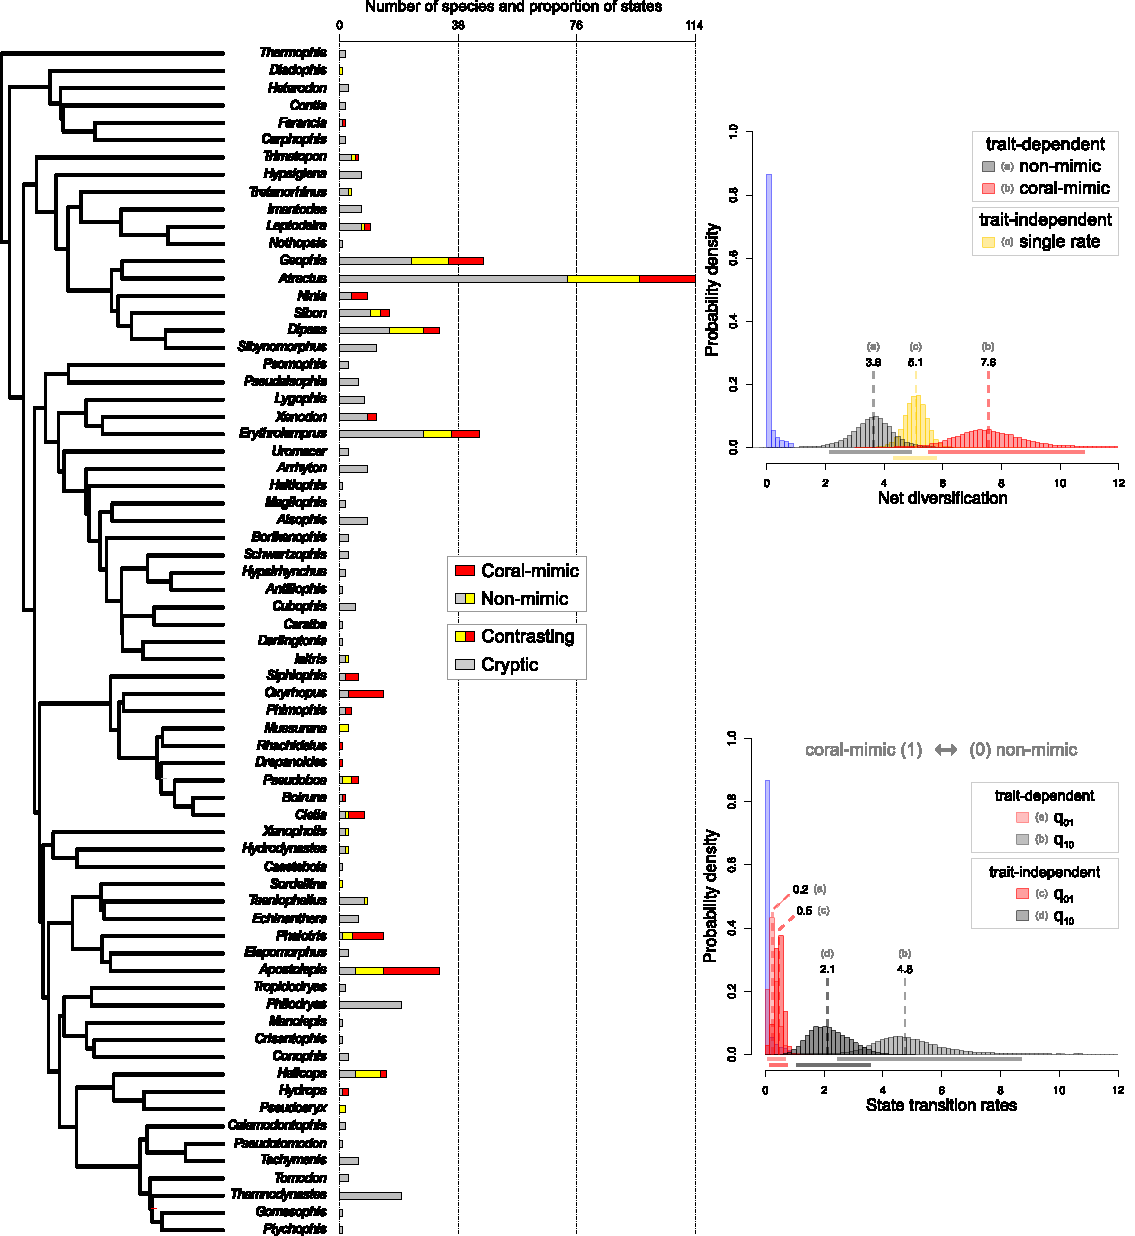
\includegraphics[scale=0.86]{Ch1_Figure_1_updated}
	\caption[Genus-level maximum clade credibility (MCC) tree of the family Dipsadidae showing the number of species assigned to each color category and posterior distribution of parameter estimates for the BiSSE model.]{Genus-level maximum clade credibility (MCC) tree of the family Dipsadidae showing the number of species assigned to each color category and posterior distribution of parameter estimates for the BiSSE model. Each color of the stacked bar chart (center) correspond to different elements of the color patterns in the group; species that do not show contrasting color patterns (i.e., cryptic coloration) are shown in gray, species with contrasting color patterns but that are not supposed mimics of coral snakes are shown in yellow, and species that show contrasting color patterns and are considered mimics of coral snakes are shown in red. (\textit{Continue on next page.})}
	\label{fig:diversity_phylo} % Figure 1.
\end{figure}

\begin{figure}[h]
  \contcaption{(\textit{Continued.}) The legend in the center of the plate applies different combinations of gray, yellow, and red to show the number of species assigned to each color category: coral-mimic (red) versus non-mimic (gray and yellow) and contrasting (yellow and red) versus cryptic (gray). Support for the genera relationships are provided in Figures \ref{fig:full_MCC1} and \ref{fig:full_MCC2}. Top-right plot shows the posterior distributions of net diversification rates under the trait-dependent (coral-mimic vs. non-mimic) and trait-independent BiSSE models. Bottom-right plot shows the posterior distributions of transition rates under the trait-dependent and trait-independent BiSSE models. Estimates are the combined posterior distribution from MCMC BiSSE runs across a pool of 100 phylogenetic trees. Prior distributions for the MCMC searches are shown in blue (unmarked distributions), the horizontal lines below each posterior distribution represent the 95\% confidence interval, and the vertical hashed lines show median values.} % Continued caption for Figure 1.
\end{figure}

\begin{figure}[h]
	\centering
	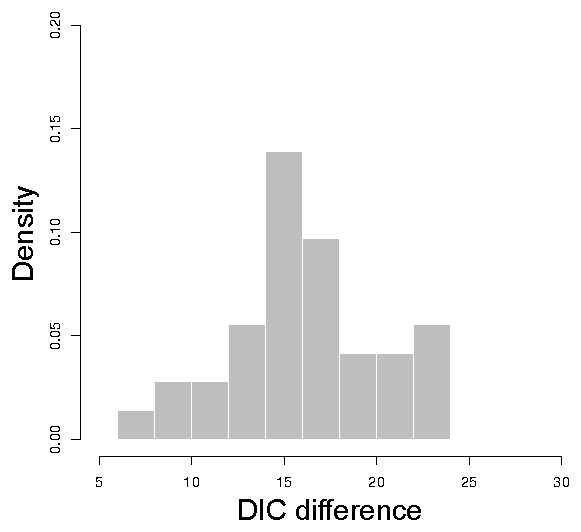
\includegraphics[scale=0.9]{Ch1_Figure_2_updated}
	\caption[Results of model selection between trait-dependent and trait-independent BiSSE models.]{Results of model selection between trait-dependent and trait-independent BiSSE models using the Bayesian Deviance Information Criteria (DIC) for the coral-mimic versus non-mimic category. Plot shows the DIC scores for the trait-dependent model (full model) subtracted from the scores for the trait-independent model (constrained model). DIC values were calculated across a pool of 100 phylogenetic trees. Large values (larger than 4 units as a rule of thumb) are expected if the trait-dependent model is to be preferred over the trait-independent model.}
	\label{fig:dic_plot} % Figure 2.
\end{figure}

\begin{figure}[h]
	\centering
	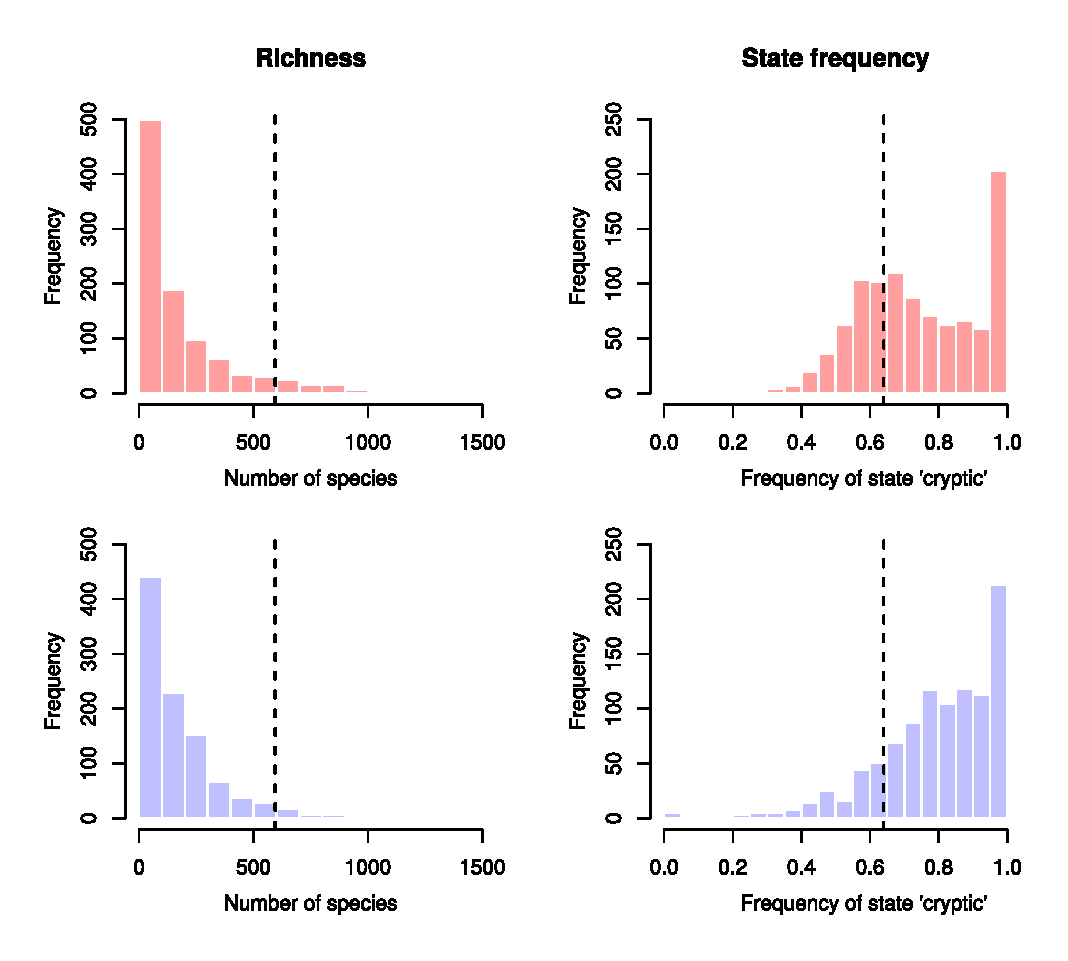
\includegraphics[scale=0.9]{Ch1_Figure_3_updated}
	\caption[Results from the posterior predictive simulations for BiSSE under the trait-dependent and the trait-independent models.]{Results from the posterior predictive simulations for BiSSE under the trait-dependent (top row - red) and the trait-independent models (bottom row - blue). Simulation parameters were drawn from the joint posterior distribution of each BiSSE model (contrasting versus cryptic color category) and phylogenetic trees. At each replicate a phylogeny was simulated under the BiSSE model until the sum of branch lengths from root to tip of the tree was equal to 1 (same as the empirical phylogeny). Left column: Total number of species in the resulting phylogenies. Vertical dashed lines show the number of species used in our analysis (594 spp.). Right column: Relative frequency of the state 0 (cryptic). Vertical dashed lines show the observed frequency of cryptic species in the data (0.64). Note that both trait-dependent and trait-independent BiSSE models show similar deviations from the observed data.}
	\label{fig:predic_BiSSE} % Figure 3.
\end{figure}

\begin{figure}[h]
	\centering
	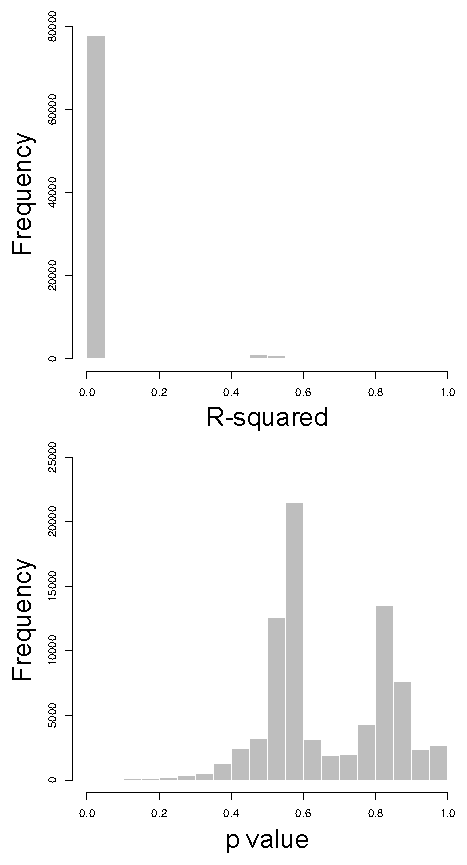
\includegraphics[scale=1.2]{Ch1_Figure_4_updated}
	\caption[Results from linear regressions between net diversification rates estimated using BAMM and the proportion of the category coral-mimic for each dipsadid genera.]{Results from linear regressions between net diversification rates estimated using BAMM (prior on expected number of shifts $\gamma$ = 1) and the proportion of the category coral-mimic for each dipsadid genera. Plots show a distribution of linear regression tests generated by repeating the analyses for each sample of the posterior distribution of the BAMM diversification estimates combined across 10 randomly sampled phylogenetic trees. Top plot shows the resulting distribution of R-squared and bottom plot the distribution of p values.}
	\label{fig:linear_BAMM} % Figure 4.
\end{figure}

\begin{figure}[h]
	\centering
	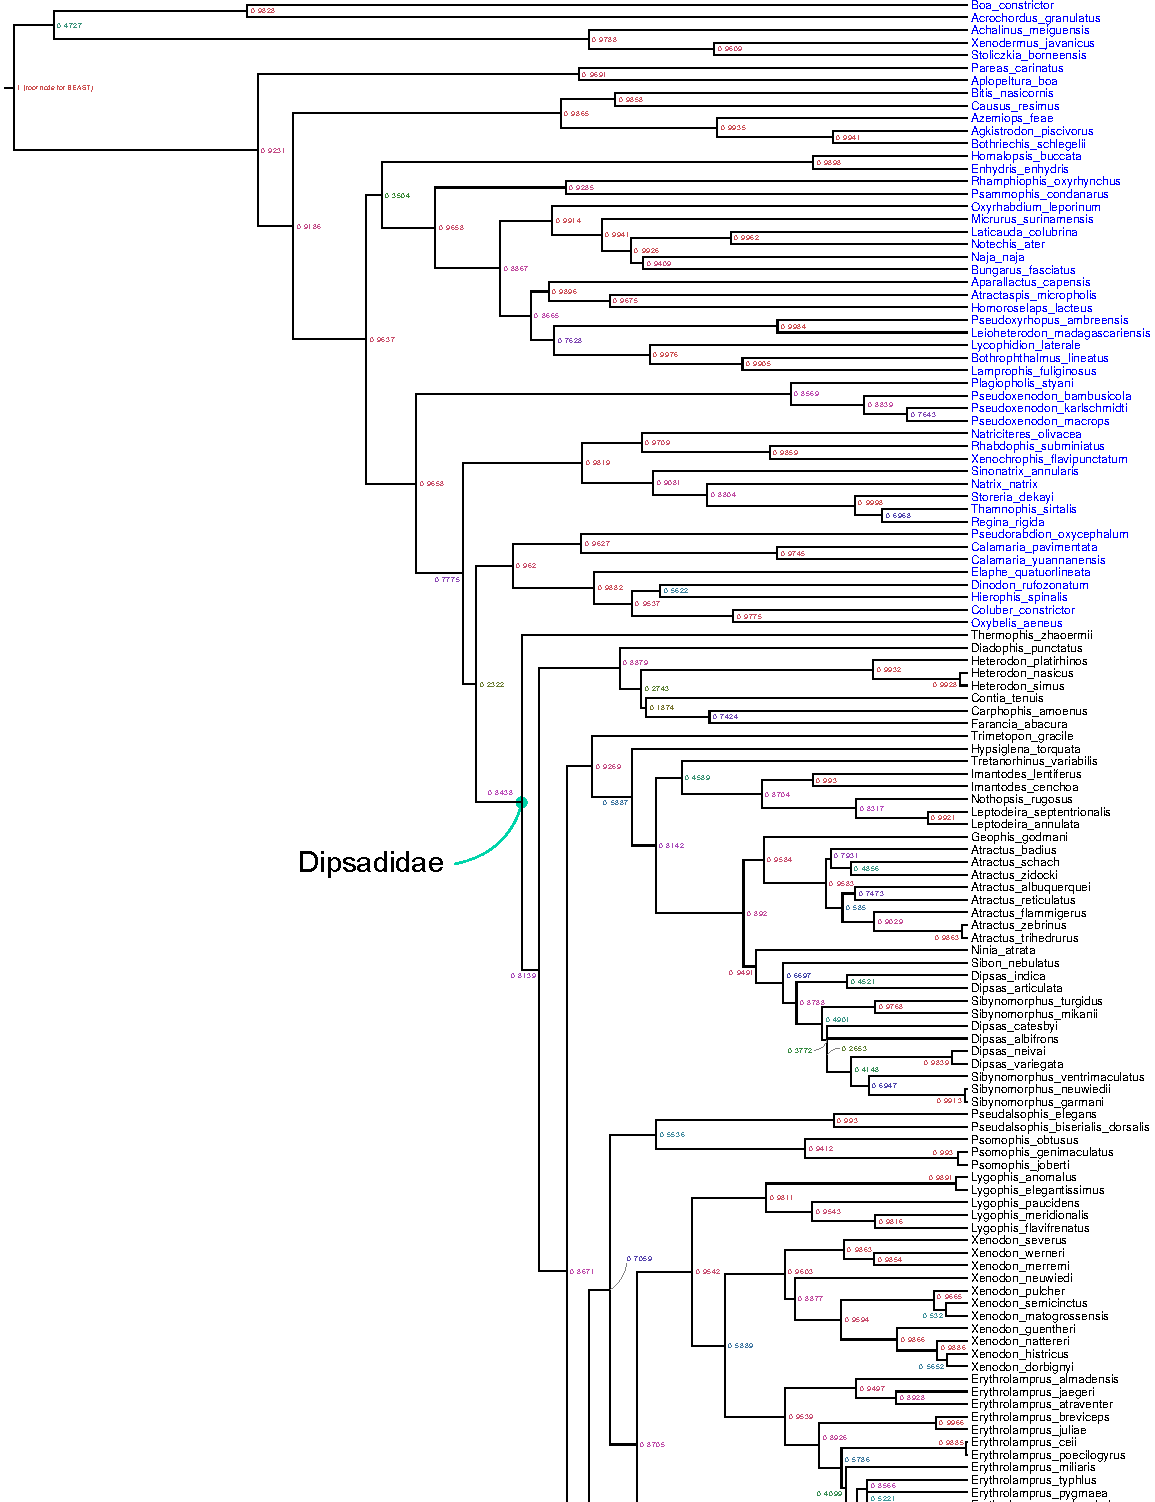
\includegraphics[scale=0.85]{Ch1_Figure_S1_updated_top}
	\caption[Maximum clade credibility tree with all species (Part 1).]{Maximum clade credibility tree with all species. Posterior probabilities are only visible on digital format. Outgroup species highlighted in blue. Continues on Figure \ref{fig:full_MCC2}.}
	\label{fig:full_MCC1} % Figure S1.
\end{figure}

\begin{figure}[h]
	\centering
	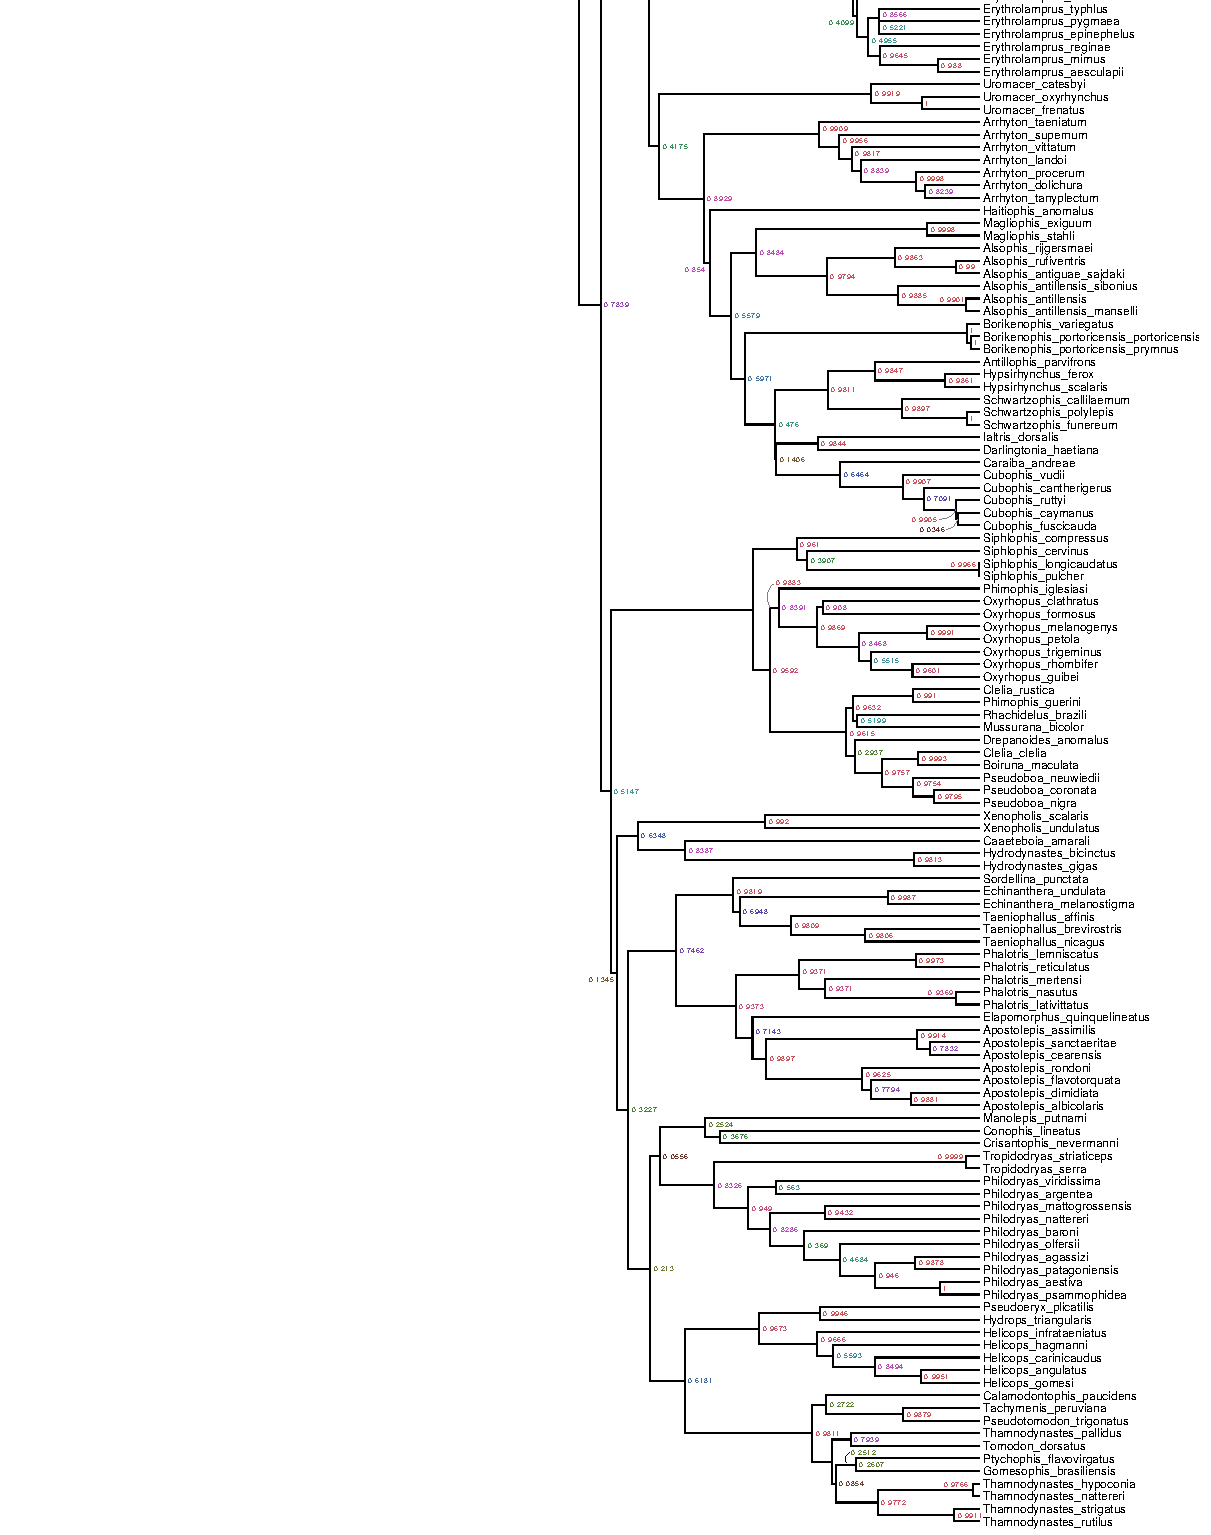
\includegraphics[scale=0.85]{Ch1_Figure_S1_updated_bottom}
	\caption[Maximum clade credibility tree with all species (Part 2).]{Maximum clade credibility tree with all species. Posterior probabilities are only visible on digital format. Continuation for Figure \ref{fig:full_MCC1}.}
	\label{fig:full_MCC2} % Figure S1.
\end{figure}

\begin{figure}[h]
	\centering
	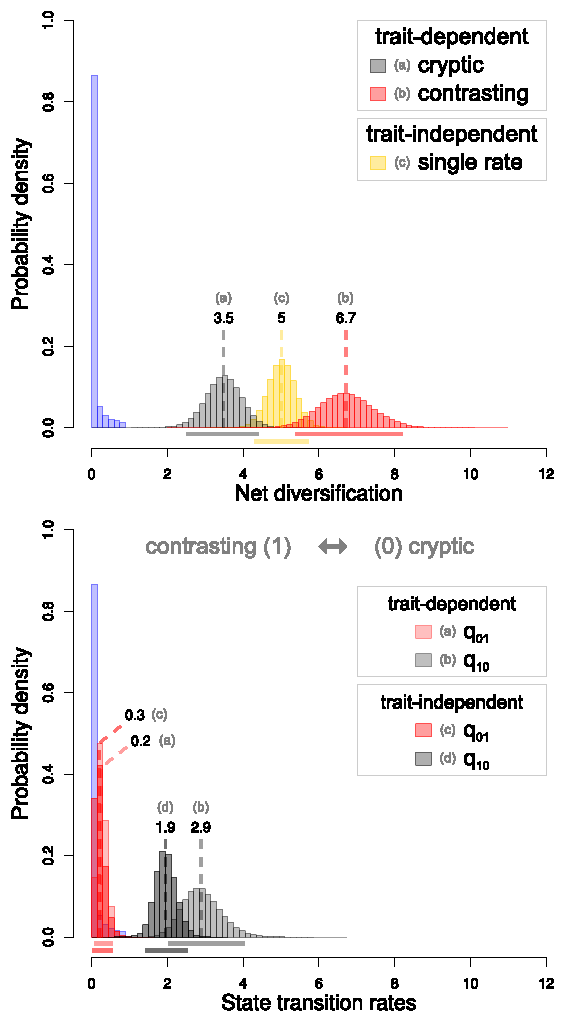
\includegraphics[scale=0.9]{Ch1_Figure_S2_updated}
	\caption[Parameter estimates for the BiSSE model under the contrasting versus cryptic color category.]{Parameter estimates for the BiSSE model under the contrasting versus cryptic color category. Top plot shows the posterior distributions of net diversification rates under the trait-dependent and trait-independent BiSSE models. Bottom plot shows the posterior distributions of transition rates under the trait-dependent and trait-independent BiSSE models. Estimates are the combined posterior distribution from MCMC BiSSE runs across a pool of 100 phylogenetic trees. Prior distributions for the MCMC searches are shown in blue (unmarked distributions), the horizontal lines below each posterior distribution represent the 95\% confidence interval, and the vertical hashed lines show median values.}
	\label{fig:par_BiSSE} % Figure S2.
\end{figure}

\begin{figure}[h]
	\centering
	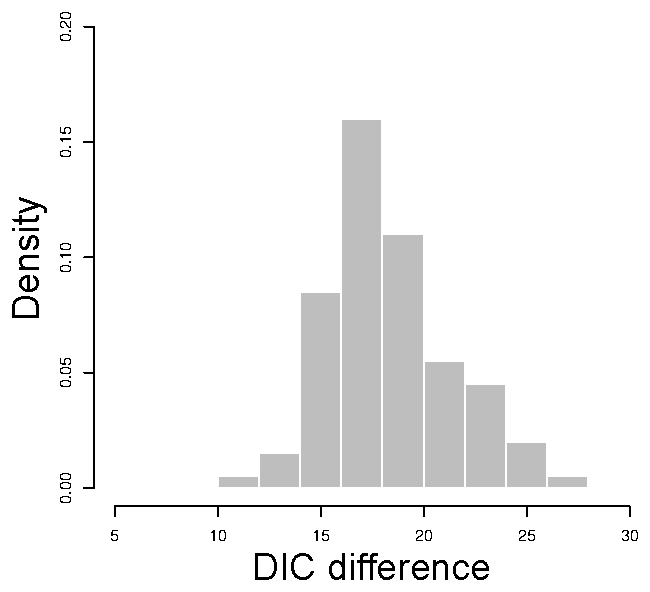
\includegraphics[scale=1]{Ch1_Figure_S3_updated}
	\caption[Results of model selection between trait-dependent and trait-independent BiSSE models.]{Results of model selection between trait-dependent and trait-independent BiSSE models using the Bayesian Deviance Information Criteria (DIC) for the contrasting versus cryptic category. Plot shows the DIC scores for the trait-dependent model (full model) subtracted from the scores for the trait-independent model (constrained model). DIC values were calculated across a pool of 100 phylogenetic trees. Large values (larger than 4 units as a rule of thumb) are expected if the trait-dependent model is to be preferred over the trait-independent model.}
	\label{fig:model_select} % Figure S3.
\end{figure}

\begin{figure}[h]
	\centering
	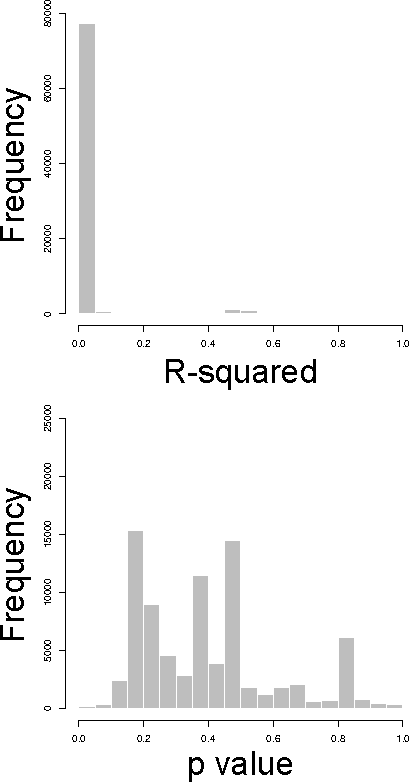
\includegraphics[scale=1.4]{Ch1_Figure_S4_updated}
	\caption[Results from linear regressions between net diversification rates estimated using BAMM.]{Results from linear regressions between net diversification rates estimated using BAMM (prior on expected number of shifts $\gamma$ = 1) and the proportion of the category contrasting for each dipsadid genera. Plots show a distribution of linear regression tests generated by repeating the analyses for each sample of the posterior distribution of the BAMM diversification estimates combined across 10 randomly sampled phylogenetic trees. Top plot shows the resulting distribution of R-squared and bottom plot the distribution of p values.}
	\label{fig:supp_linear_BAMM} % Figure S4.
\end{figure}

\begin{figure}[h]
	\centering
	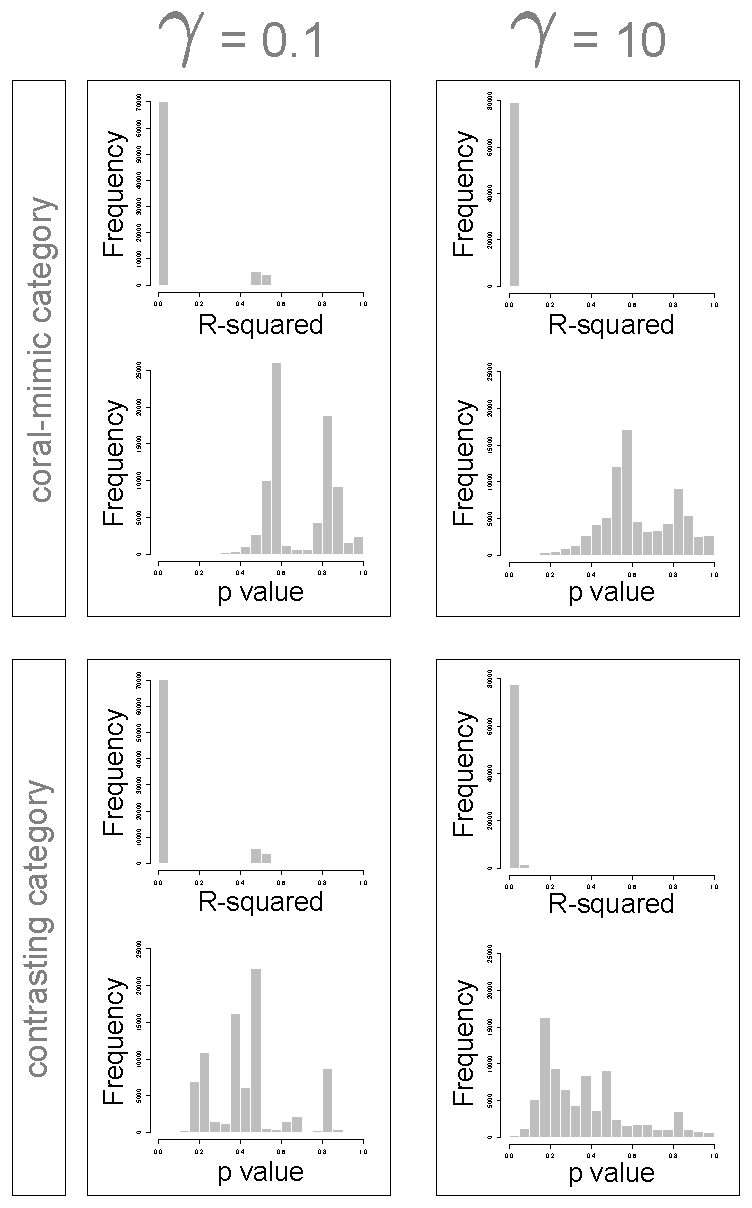
\includegraphics[scale=1.2]{Ch1_Figure_S5_updated}
%	\caption[Results from linear regressions between net diversification rates estimated using BAMM and the proportion of both color categories coral-mimic and contrasting for each dipsadid genera under different prior distributions on the number of expected rate shifts.]{Results from linear regressions between net diversification rates estimated using BAMM and the proportion of both color categories coral-mimic and contrasting for each dipsadid genera under different prior distributions on the number of expected rate shifts. Each plot show a distribution of results from linear regression tests generated by repeating the analyses for each sample of the posterior distribution of BAMM diversification estimates combined across 10 randomly sampled phylogenetic trees. The top plot within each treatment show the resulting distribution of R-squared and bottom plot the distribution of p values. Top row are results using the color category coral-mimic and bottom row using category contrasting. Results on the left column were based on a prior distribution for the expected number of shifts ( $\gamma$ ) equal to 0.1 and on the right column equal to 10.}
%	\label{fig:prior_linear_BAMM} % Figure S5.
\end{figure}
\clearpage % insert a page break
\captionof{figure}[Results from linear regressions between net diversification rates estimated using BAMM and the proportion of both color categories coral-mimic and contrasting for each dipsadid genera under different prior distributions on the number of expected rate shifts.]{Results from linear regressions between net diversification rates estimated using BAMM and the proportion of both color categories coral-mimic and contrasting for each dipsadid genera under different prior distributions on the number of expected rate shifts. Each plot show a distribution of results from linear regression tests generated by repeating the analyses for each sample of the posterior distribution of BAMM diversification estimates combined across 10 randomly sampled phylogenetic trees. The top plot within each treatment show the resulting distribution of R-squared and bottom plot the distribution of p values. Top row are results using the color category coral-mimic and bottom row using category contrasting. Results on the left column were based on a prior distribution for the expected number of shifts ( $\gamma$ ) equal to 0.1 and on the right column equal to 10.}
\label{fig:prior_linear_BAMM} % Figure S5.